\documentclass[12pt]{article}

\usepackage{fontawesome}
\usepackage{hyperref}
\usepackage{xurl}
\usepackage{graphicx}
\usepackage{float}
\usepackage[tagged, highstructure]{accessibility}
\usepackage{bookmark}
\usepackage{enumitem}

\hypersetup{
    colorlinks=false,
    pdfborder={0 0 0},
    pdftitle={Data Collection Lab},
    pdfauthor={Adrianna Holden-Gouveia},
    pdfsubject={Introduction to Data - Lab Assignment},
    pdflang={en-US},
    pdfkeywords={data collection, data analysis, statistics}
}

% Configure PDF bookmarks for navigation
\bookmarksetup{
    numbered,
    open,
}

% Configure list spacing for better accessibility
\setlist{nosep}



\title{Data Collection}
\author{
        Adrianna Holden-Gouveia \\
        Website: \href{https://aholdengouveia.name}{aholdengouveia.name}\\
        \date{\vspace{-5ex}}
        %Email: \href{mailto:admin@aholdengouveia.name}{admin@aholdengouveia.name} \\
        \faGithub {: aholdengouveia} \\
        %\faTwitter {: aholdengouveia} \\
        }

%S\date{\today}


\begin{document}    

\maketitle

%\begin{abstract}
%This is a template for Linux Administration Lab work
%\end{abstract}
%\tableofcontents


\section*{Accessibility Notice}
This document is also available in HTML format at:

Link: \href{https://aholdengouveia.name/IntroData/labs/whatisdata.html}{\textbf{\nolinkurl{https://aholdengouveia.name/IntroData/labs/whatisdata.html}}}

The HTML version provides enhanced accessibility features including keyboard navigation, screen reader support, responsive design, dark mode support, and high contrast options.

\section*{Objectives:}
    The goal of this lab assignment is for students to distinguish between data and information using real-world examples. Through practical scenarios and observations, students will explore the transformation of raw data into meaningful information.  Students will also practice gathering data and finding good sources of data.

\section*{Data Collection}

References, a video, a PowerPoint and some notes are available at my website Link: \href{https://www.aholdengouveia.name/IntroData/dataforeveryone.html}{\textbf{\nolinkurl{https://www.aholdengouveia.name/IntroData/dataforeveryone.html}}}

Pick one of the following topics and collect some data about it. You can use a text editor or spreadsheet to collect your data. Think about what is good data to collect for your topic, and what your column and row names should be.
\begin{itemize}
    \item Sports Statistics
    \item Weather Data
    \item Collectible Card Game such as Magic: The Gathering, or Vampire: The Masquerade
    \item Video game stats for items or characters in the game
    \item Collectibles such as figurines for Warhammer or D\&D
\end{itemize}
You may pick another topic not listed above, but it can't be books.

\subsection*{Data Requirements}
\begin{itemize}
    \item At least 100 records (rows), and no more than 1000
    \item At least 7 labeled columns per record
    \item Your data can include numbers, figures, text, or any relevant data points.
    \item Keep it raw. Raw data should be unprocessed and unorganized. This means you shouldn't try to manipulate the data yet or do anything to it besides make sure it's in a table with labels. It's ok to have errors and duplications and other things like that at this stage.
\end{itemize}

\subsection*{Sample Data and Where to Find Data}
A sample of book data, 100bestbooks.csv, is linked here Link: \href{https://www.aholdengouveia.name/IntroData/labs/100bestbooks.csv}{\textbf{\nolinkurl{https://www.aholdengouveia.name/IntroData/labs/100bestbooks.csv}}}

The sample data was collected from Link: \href{https://zenodo.org/records/4265096}{\textbf{\nolinkurl{https://zenodo.org/records/4265096}}}

There are some suggestions for where you can get data sets on the Resources page Link: \href{https://www.aholdengouveia.name/IntroData/Resources.html}{\textbf{\nolinkurl{https://www.aholdengouveia.name/IntroData/Resources.html}}}

\subsection*{Questions}
    \begin{enumerate}
        \item Your source
        \begin{enumerate}
            \item Where did your data come from, and how did you find it? Include links to any websites you used.
            \item Why do you think this is a good source of data?
        \end{enumerate}
        \item Why did you decide on this type of data?
        \item Data and information
        \begin{enumerate}
            \item Give 2 examples of raw data from your data set.
            \item For each example, what information can you get from it? Explain how the raw data becomes meaningful information.
        \end{enumerate}
        \item What trends or patterns can be observed?
        \item Are there any outliers or significant data points?
        \item What are at least 3 things you've noticed about your data?
        \item How did you decide on your column naming?
        \item What was the biggest challenge you had while collecting your data?
        \item Can you see any obvious mistakes or issues with your data? If yes, what are they?
        \item What do you think would be the best way to present this data to others?
        \item What, if anything, have you learned from collecting this data?
        \item If you had to collect this data again, what might you change?
    \end{enumerate}

\subsection*{Visualizations}
    \begin{enumerate}
        \item Your visualization
        \begin{enumerate}
            \item Create at least 1 visualization of your data, as a whole or parts depending on what you think is best.
            \item Take a screenshot of your visualization.
            \item Explain why you chose what you did.
        \end{enumerate}
        \item AI visualization
        \begin{enumerate}
            \item Use an AI of your choice to create a visualization of your data.
            \item Take a screenshot of the AI's visualization.
            \item Which AI did you use, and why did you pick that one?
            \item How does the AI's visualization compare to yours? Which one shows your data better, and why?
        \end{enumerate}
        \item If you prefer not to use an AI, do this instead of question 2: find a published visualization.
        \begin{enumerate}
            \item Find a visualization that someone else has published of data similar to yours, for example on a sports statistics site, a weather service, or a game wiki. Include the link.
            \item Take a screenshot of the published visualization.
            \item Why do you think this is a good source?
            \item How does the published visualization compare to yours? Which one shows the data better, and why?
        \end{enumerate}
    \end{enumerate}

\subsection*{Screenshots}
You need 3 screenshots: your data, your visualization, and either the AI's visualization (question 2) or the published visualization (question 3).

Each screenshot should have your name, term, and year.  One of the easiest ways to do that is make a text document with your name and term/year on your computer and save it to use all term. Any screenshots that don't include this information won't be counted.

\begin{figure}[H]
    \centering
    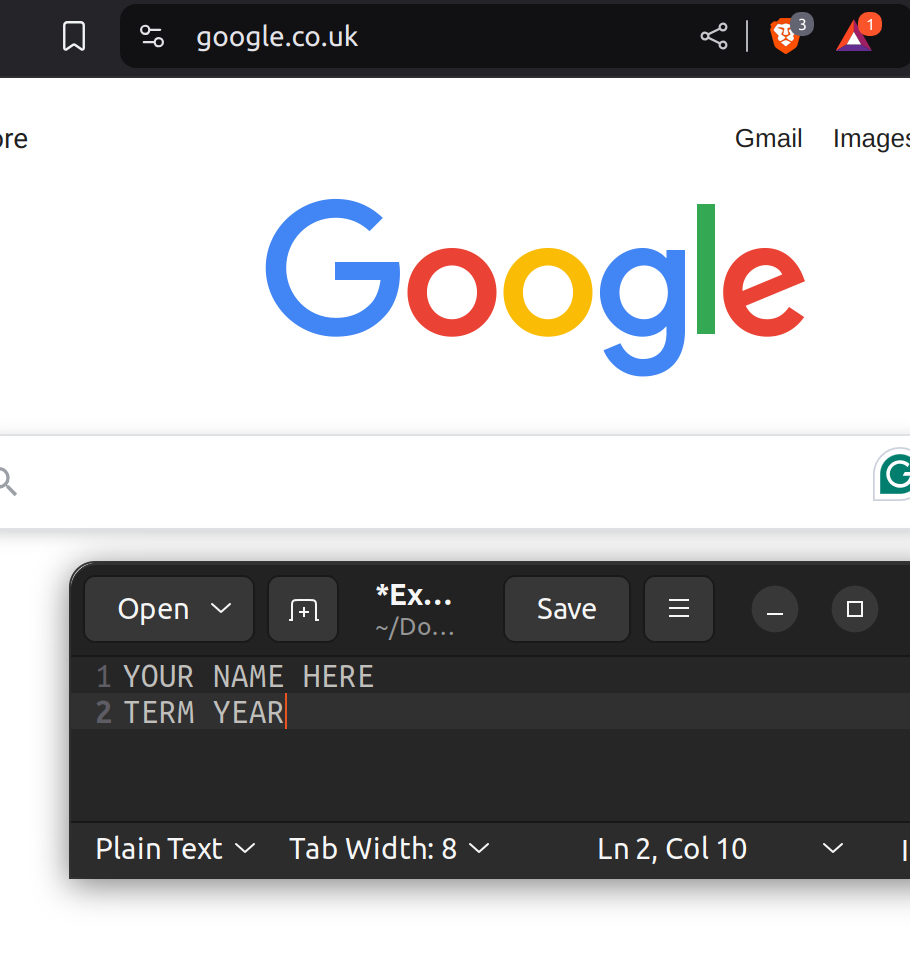
\includegraphics[scale=.2]{ExampleScreenshot.png}
    \caption{This is an image of what each of your screenshots should look like}
    \alt{Example screenshot: a web browser showing the Google home page, with a small text editor window in front of it that says YOUR NAME HERE and TERM YEAR}
\end{figure}

\section*{Deliverables:}
This lab should have 2 files submitted.
\begin{enumerate}
    \item Your raw data, as either a CSV or spreadsheet
    \item One document, clearly labeled, with:
    \begin{enumerate}
        \item Your answers to the Questions, labeled with their question numbers
        \item Your answers to the Visualizations section
        \item All 3 screenshots
    \end{enumerate}
\end{enumerate}
\end{document}